\documentclass{article}
\usepackage{graphicx}
\title{Gargi: LOML}
\author{mili}
\date{December 2024}

\begin{document}
\maketitle

\section{Introduction}
Gargi is such a wonderful person, I am so lucky to have met her. She is kind, brave, humble and playful, funny, warm personality. I don't know, this is not a tick the box to choose someone, before knowing these qualities I just fell for her, I didn't even have her pics. It's just that my heart went after her and I don't know why, it's a strange thing for sure. But I am so happy that it went to her. $h^2 = @6$

\% \$

$\sigma \pi$

\begin{equation}
    \sqrt{5} + \frac{1}{5}\sigma + 5 = \alpha + 2
\end{equation}

\begin{itemize}
    \item first point
    \item second point
    \item third point
\end{itemize}

\begin{enumerate}
    \item hello
    \item high
    \item gargiiiiiiiiii
\end{enumerate}

aorinstaiorsntoianrstoinarotinarint

\subsection{graphic}
lorem lorem lorem lorem lorem lorem lorem lorem lorem lorem lorem lorem lorem lorem lorem lorem lorem lorem lorem lorem lorem lorem lorem

\begin{figure}
    \centering
    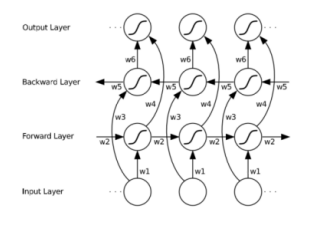
\includegraphics{assets/image1.png}
    \caption{an image caption}
    \label{fig: nothing to see here}
\end{figure}

\subsubsection{graphic2}
Lorem ipsum dolor sit amet, consectetur adipiscing elit. Sed do eiusmod tempor incididunt ut labore et dolore magna aliqua. Ut enim ad minim veniam, quis nostrud exercitation ullamco laboris nisi ut aliquip ex ea commodo consequat. Duis aute irure dolor in reprehenderit in voluptate velit esse cillum dolore eu fugiat nulla pariatur. Excepteur sint occaecat cupidatat non proident, sunt in culpa qui officia deserunt mollit anim id est laborum.

Curabitur pretium tincidunt lacus. Nulla gravida orci a odio. Nullam varius, turpis et commodo pharetra, est eros bibendum elit,

\begin{table}[h]
    \centering
    \caption{A table heading}
    \begin{tabular}{|c|c|c|}
        \hline
        \multicolumn{2}{|c|}{First column} & \multicolumn{1}{|c|}{Second column}                                    \\
        \hline
        Apple                              & Mango                               & \multicolumn{1}{|c|}{volleyball} \\
        \hline
        Apple                              & Mango                               & \multicolumn{1}{|c|}{volleyball} \\
        \hline
    \end{tabular}
\end{table}

\end{document}